% The cloud-segmentation U-Net of skypass/ml/cloudcam.py (base 16 channels, input 160 px).
% Built by experiments/diagrams/build_diagrams.py. Palette: Okabe-Ito.
\documentclass[border=4pt]{standalone}
\usepackage{tikz}
\usetikzlibrary{arrows.meta, calc, positioning}
\definecolor{enc}{HTML}{0072B2}
\definecolor{dec}{HTML}{E69F00}
\definecolor{mid}{HTML}{CC79A7}
\definecolor{pool}{HTML}{D55E00}
\definecolor{up}{HTML}{009E73}
\definecolor{skip}{HTML}{777777}
\definecolor{sky}{HTML}{56B4E9}
\begin{document}
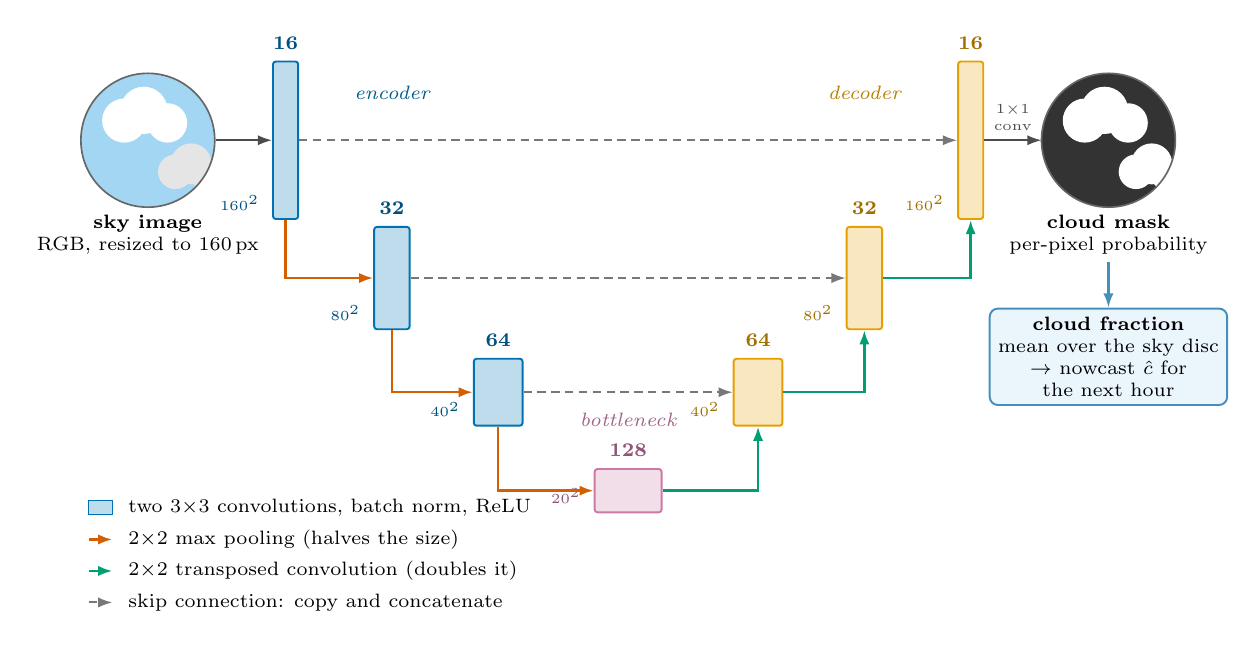
\begin{tikzpicture}[font=\scriptsize, >={Latex[length=1.8mm, width=1.3mm]}]
% block: \blk{name}{x}{y}{width}{height}{colour}{channels}{size}
\newcommand{\blk}[8]{%
  \node[draw=#6, fill=#6!25, line width=0.7pt, minimum width=#4cm, minimum height=#5cm,
        inner sep=0pt, rounded corners=1pt] (#1) at (#2,#3) {};
  \node[font=\scriptsize\bfseries, text=#6!70!black, above=0.5pt of #1] {#7};
  \node[font=\tiny, text=#6!70!black, anchor=south east] at ($(#1.south west)+(-0.04,0)$) {#8};}
% ---------------------------------------------------------------- input image
\begin{scope}
  \fill[sky!55] (-1.75,0) circle (0.85);
  \clip (-1.75,0) circle (0.85);
  \fill[white] (-2.05,0.25) circle (0.28) (-1.8,0.38) circle (0.3) (-1.5,0.22) circle (0.25);
  \fill[white!90!black] (-1.4,-0.4) circle (0.22) (-1.2,-0.3) circle (0.26) (-1.0,-0.45) circle (0.2);
\end{scope}
\draw[black!60, line width=0.6pt] (-1.75,0) circle (0.85);
\node[align=center, font=\scriptsize] at (-1.75,-1.2) {\textbf{sky image}\\RGB, resized to 160\,px};
% ---------------------------------------------------------------- encoder
\blk{e1}{0}{0}{0.32}{2.0}{enc}{16}{160\textsuperscript{2}}
\blk{e2}{1.35}{-1.75}{0.45}{1.3}{enc}{32}{80\textsuperscript{2}}
\blk{e3}{2.7}{-3.2}{0.62}{0.85}{enc}{64}{40\textsuperscript{2}}
\blk{m}{4.35}{-4.45}{0.85}{0.55}{mid}{128}{20\textsuperscript{2}}
% ---------------------------------------------------------------- decoder
\blk{d3}{6.0}{-3.2}{0.62}{0.85}{dec}{64}{40\textsuperscript{2}}
\blk{d2}{7.35}{-1.75}{0.45}{1.3}{dec}{32}{80\textsuperscript{2}}
\blk{d1}{8.7}{0}{0.32}{2.0}{dec}{16}{160\textsuperscript{2}}
% ---------------------------------------------------------------- arrows
\draw[->, black!70, line width=0.7pt] (-0.88,0) -- (e1.west);
\draw[->, pool, line width=0.9pt] (e1.south) |- (e2.west);
\draw[->, pool, line width=0.9pt] (e2.south) |- (e3.west);
\draw[->, pool, line width=0.9pt] (e3.south) |- (m.west);
\draw[->, up, line width=0.9pt] (m.east) -| (d3.south);
\draw[->, up, line width=0.9pt] (d3.east) -| (d2.south);
\draw[->, up, line width=0.9pt] (d2.east) -| (d1.south);
\draw[->, skip, densely dashed, line width=0.7pt] (e1.east) -- (d1.west);
\draw[->, skip, densely dashed, line width=0.7pt] (e2.east) -- (d2.west);
\draw[->, skip, densely dashed, line width=0.7pt] (e3.east) -- (d3.west);
% ---------------------------------------------------------------- output mask
\begin{scope}
  \fill[black!80] (10.45,0) circle (0.85);
  \clip (10.45,0) circle (0.85);
  \fill[white] (10.15,0.25) circle (0.28) (10.4,0.38) circle (0.3) (10.7,0.22) circle (0.25);
  \fill[white] (10.8,-0.4) circle (0.22) (11.0,-0.3) circle (0.26) (11.2,-0.45) circle (0.2);
\end{scope}
\draw[black!60, line width=0.6pt] (10.45,0) circle (0.85);
\draw[->, black!70, line width=0.7pt] (d1.east) -- node[above, font=\tiny, align=center] {1$\times$1\\conv} (9.6,0);
\node[align=center, font=\scriptsize] at (10.45,-1.2) {\textbf{cloud mask}\\per-pixel probability};
\node[draw=sky!80!black, fill=sky!12, rounded corners=3pt, align=center, font=\scriptsize,
      line width=0.7pt, inner sep=3pt] (frac) at (10.45,-2.75)
     {\textbf{cloud fraction}\\mean over the sky disc\\$\to$ nowcast $\hat c$ for\\the next hour};
\draw[->, sky!80!black, line width=0.8pt] (10.45,-1.55) -- (frac.north);
% ---------------------------------------------------------------- legend
\begin{scope}[shift={(-2.5,-4.75)}]
  \draw[fill=enc!25, draw=enc] (0,0) rectangle (0.3,0.18);
  \node[anchor=west] at (0.38,0.09) {two 3$\times$3 convolutions, batch norm, ReLU};
  \draw[->, pool, line width=0.9pt] (0,-0.32) -- (0.3,-0.32);
  \node[anchor=west] at (0.38,-0.32) {2$\times$2 max pooling (halves the size)};
  \draw[->, up, line width=0.9pt] (0,-0.72) -- (0.3,-0.72);
  \node[anchor=west] at (0.38,-0.72) {2$\times$2 transposed convolution (doubles it)};
  \draw[->, skip, densely dashed, line width=0.7pt] (0,-1.12) -- (0.3,-1.12);
  \node[anchor=west] at (0.38,-1.12) {skip connection: copy and concatenate};
\end{scope}
\node[font=\scriptsize\itshape, text=enc!80!black] at (1.35,0.6) {encoder};
\node[font=\scriptsize\itshape, text=dec!80!black] at (7.35,0.6) {decoder};
\node[font=\scriptsize\itshape, text=mid!80!black, align=center] at (4.35,-3.55) {bottleneck};
\end{tikzpicture}
\end{document}
